% Options for packages loaded elsewhere
\PassOptionsToPackage{unicode}{hyperref}
\PassOptionsToPackage{hyphens}{url}
%
\documentclass[
]{article}
\usepackage{amsmath,amssymb}
\usepackage{iftex}
\ifPDFTeX
  \usepackage[T1]{fontenc}
  \usepackage[utf8]{inputenc}
  \usepackage{textcomp} % provide euro and other symbols
\else % if luatex or xetex
  \usepackage{unicode-math} % this also loads fontspec
  \defaultfontfeatures{Scale=MatchLowercase}
  \defaultfontfeatures[\rmfamily]{Ligatures=TeX,Scale=1}
\fi
\usepackage{lmodern}
\ifPDFTeX\else
  % xetex/luatex font selection
\fi
% Use upquote if available, for straight quotes in verbatim environments
\IfFileExists{upquote.sty}{\usepackage{upquote}}{}
\IfFileExists{microtype.sty}{% use microtype if available
  \usepackage[]{microtype}
  \UseMicrotypeSet[protrusion]{basicmath} % disable protrusion for tt fonts
}{}
\makeatletter
\@ifundefined{KOMAClassName}{% if non-KOMA class
  \IfFileExists{parskip.sty}{%
    \usepackage{parskip}
  }{% else
    \setlength{\parindent}{0pt}
    \setlength{\parskip}{6pt plus 2pt minus 1pt}}
}{% if KOMA class
  \KOMAoptions{parskip=half}}
\makeatother
\usepackage{xcolor}
\usepackage[margin=1in]{geometry}
\usepackage{color}
\usepackage{fancyvrb}
\newcommand{\VerbBar}{|}
\newcommand{\VERB}{\Verb[commandchars=\\\{\}]}
\DefineVerbatimEnvironment{Highlighting}{Verbatim}{commandchars=\\\{\}}
% Add ',fontsize=\small' for more characters per line
\usepackage{framed}
\definecolor{shadecolor}{RGB}{248,248,248}
\newenvironment{Shaded}{\begin{snugshade}}{\end{snugshade}}
\newcommand{\AlertTok}[1]{\textcolor[rgb]{0.94,0.16,0.16}{#1}}
\newcommand{\AnnotationTok}[1]{\textcolor[rgb]{0.56,0.35,0.01}{\textbf{\textit{#1}}}}
\newcommand{\AttributeTok}[1]{\textcolor[rgb]{0.13,0.29,0.53}{#1}}
\newcommand{\BaseNTok}[1]{\textcolor[rgb]{0.00,0.00,0.81}{#1}}
\newcommand{\BuiltInTok}[1]{#1}
\newcommand{\CharTok}[1]{\textcolor[rgb]{0.31,0.60,0.02}{#1}}
\newcommand{\CommentTok}[1]{\textcolor[rgb]{0.56,0.35,0.01}{\textit{#1}}}
\newcommand{\CommentVarTok}[1]{\textcolor[rgb]{0.56,0.35,0.01}{\textbf{\textit{#1}}}}
\newcommand{\ConstantTok}[1]{\textcolor[rgb]{0.56,0.35,0.01}{#1}}
\newcommand{\ControlFlowTok}[1]{\textcolor[rgb]{0.13,0.29,0.53}{\textbf{#1}}}
\newcommand{\DataTypeTok}[1]{\textcolor[rgb]{0.13,0.29,0.53}{#1}}
\newcommand{\DecValTok}[1]{\textcolor[rgb]{0.00,0.00,0.81}{#1}}
\newcommand{\DocumentationTok}[1]{\textcolor[rgb]{0.56,0.35,0.01}{\textbf{\textit{#1}}}}
\newcommand{\ErrorTok}[1]{\textcolor[rgb]{0.64,0.00,0.00}{\textbf{#1}}}
\newcommand{\ExtensionTok}[1]{#1}
\newcommand{\FloatTok}[1]{\textcolor[rgb]{0.00,0.00,0.81}{#1}}
\newcommand{\FunctionTok}[1]{\textcolor[rgb]{0.13,0.29,0.53}{\textbf{#1}}}
\newcommand{\ImportTok}[1]{#1}
\newcommand{\InformationTok}[1]{\textcolor[rgb]{0.56,0.35,0.01}{\textbf{\textit{#1}}}}
\newcommand{\KeywordTok}[1]{\textcolor[rgb]{0.13,0.29,0.53}{\textbf{#1}}}
\newcommand{\NormalTok}[1]{#1}
\newcommand{\OperatorTok}[1]{\textcolor[rgb]{0.81,0.36,0.00}{\textbf{#1}}}
\newcommand{\OtherTok}[1]{\textcolor[rgb]{0.56,0.35,0.01}{#1}}
\newcommand{\PreprocessorTok}[1]{\textcolor[rgb]{0.56,0.35,0.01}{\textit{#1}}}
\newcommand{\RegionMarkerTok}[1]{#1}
\newcommand{\SpecialCharTok}[1]{\textcolor[rgb]{0.81,0.36,0.00}{\textbf{#1}}}
\newcommand{\SpecialStringTok}[1]{\textcolor[rgb]{0.31,0.60,0.02}{#1}}
\newcommand{\StringTok}[1]{\textcolor[rgb]{0.31,0.60,0.02}{#1}}
\newcommand{\VariableTok}[1]{\textcolor[rgb]{0.00,0.00,0.00}{#1}}
\newcommand{\VerbatimStringTok}[1]{\textcolor[rgb]{0.31,0.60,0.02}{#1}}
\newcommand{\WarningTok}[1]{\textcolor[rgb]{0.56,0.35,0.01}{\textbf{\textit{#1}}}}
\usepackage{graphicx}
\makeatletter
\newsavebox\pandoc@box
\newcommand*\pandocbounded[1]{% scales image to fit in text height/width
  \sbox\pandoc@box{#1}%
  \Gscale@div\@tempa{\textheight}{\dimexpr\ht\pandoc@box+\dp\pandoc@box\relax}%
  \Gscale@div\@tempb{\linewidth}{\wd\pandoc@box}%
  \ifdim\@tempb\p@<\@tempa\p@\let\@tempa\@tempb\fi% select the smaller of both
  \ifdim\@tempa\p@<\p@\scalebox{\@tempa}{\usebox\pandoc@box}%
  \else\usebox{\pandoc@box}%
  \fi%
}
% Set default figure placement to htbp
\def\fps@figure{htbp}
\makeatother
\setlength{\emergencystretch}{3em} % prevent overfull lines
\providecommand{\tightlist}{%
  \setlength{\itemsep}{0pt}\setlength{\parskip}{0pt}}
\setcounter{secnumdepth}{-\maxdimen} % remove section numbering
\usepackage{bookmark}
\IfFileExists{xurl.sty}{\usepackage{xurl}}{} % add URL line breaks if available
\urlstyle{same}
\hypersetup{
  pdftitle={Stat 201: Exploratory Data Analysis in R},
  hidelinks,
  pdfcreator={LaTeX via pandoc}}

\title{Stat 201: Exploratory Data Analysis in R}
\author{}
\date{\vspace{-2.5em}}

\begin{document}
\maketitle

{
\setcounter{tocdepth}{2}
\tableofcontents
}
\phantomsection\label{boxedtext}
\textbf{Learning Objectives}

\begin{itemize}
\tightlist
\item
  Become comfortable with the RStudio interface.
\item
  Understand how to record written explanations and code chunks in an
  RMarkdown file and \texttt{knit} the file into a report.
\item
  Run some fun, basic commands in R.
\item
  Load our first dataset into R: use this dataset to review basic
  concepts about exploratory data analysis.
\end{itemize}

\subsection{Why R?}\label{why-r}

R is an incredibly popular programming language for data analysis. It is
used by statisticians but also by scientists in biology, psychology,
economics, chemistry, etc. R is fully featured and very powerful, and
unlike Stata or SaaS, it is \emph{free and open source}. This means that
you can continue to use it for free after you finish this class, and
beyond. Additionally, R is \emph{extensible}. When a statistician
develops a new method, or when a scientist decides that they need a
specific tool to analyze their specific data, they (or someone who wants
to use it in R) will often implement the method as a collection of
functions in R called a \emph{package}. Other individuals who want to
use the method or conduct a similar type of data analysis can download
the package and use these functions without needing to rewrite all of
the code themselves. The Comprehensive R Archive Network, or
\textbf{CRAN}, contains over 13,000
\href{https://cran.r-project.org/web/packages/}{contributed packages}.

\section{Getting Started}\label{getting-started}

Hopefully you were able to download R and RStudio by following the
instructions on GLOW. If so, go ahead and launch RStudio. You should see
a window that looks like the image shown below.

\pandocbounded{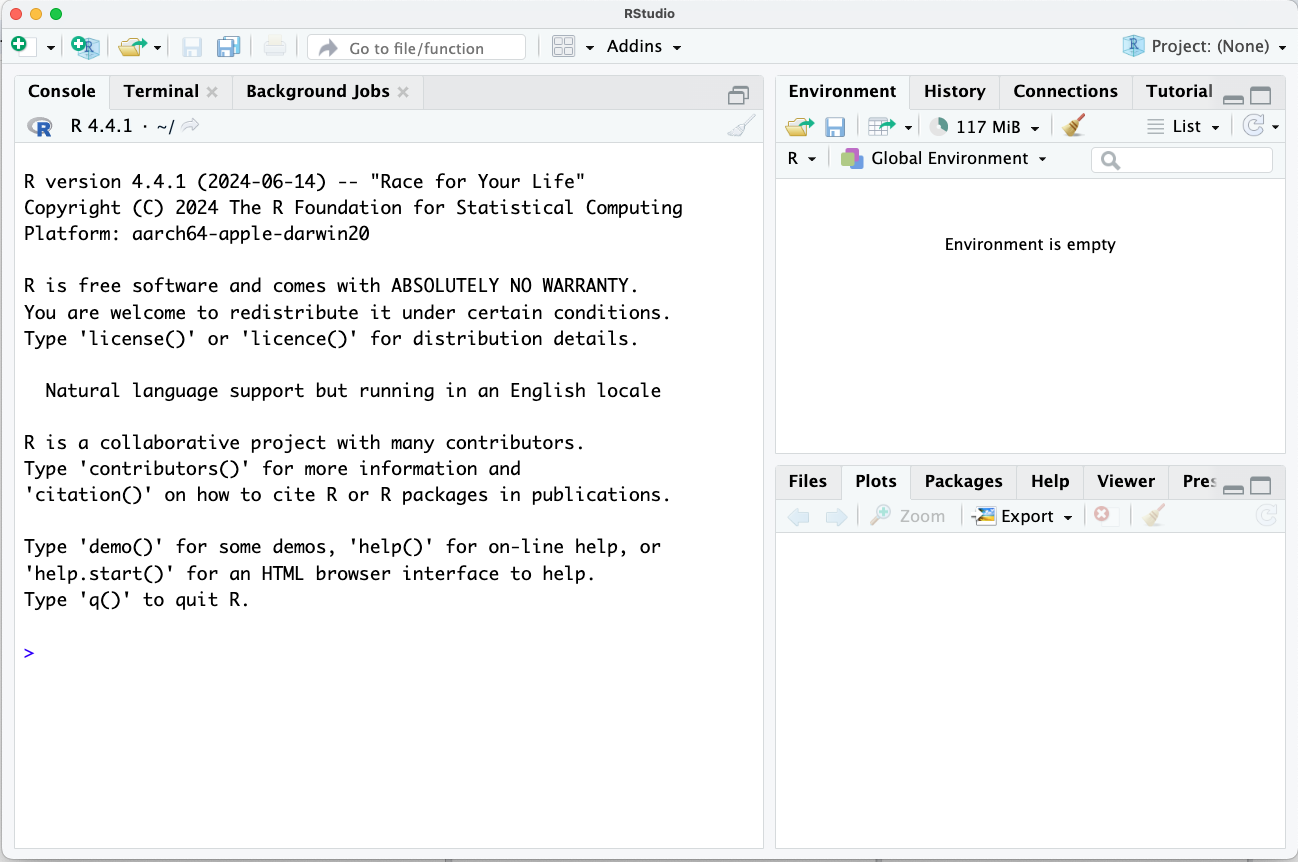
\includegraphics[keepaspectratio]{R_interface.png}}

The panel on the lower left is where the action happens. It's called the
\emph{console}. Every time you launch RStudio, it will have the same
text at the top of the console telling you the version of R that you're
running. Below that information you will see the symbol \(>\). This is
called the \emph{prompt}: it is a request for a command. Initially,
interacting with R is all about typing commands into the console and
interpreting the output.

The panel in the upper right contains your \emph{environment}, which
will show you all of your named variables and datasets once you
create/load them. You can also view a \emph{history} of all commands you
have previously entered in the console.

Any plots that you generate will show up in the panel in the lower right
corner. This is also where you can browse your files, access help,
manage packages, etc.

\begin{center}\rule{0.5\linewidth}{0.5pt}\end{center}

\subsubsection{Loading Packages}\label{loading-packages}

R is an open-source programming language, meaning that users can
contribute packages that make our lives easier, and we can use them for
free. For many labs in the future we will use the following R packages:

\begin{itemize}
\tightlist
\item
  The suite of \textbf{tidyverse} packages: for data wrangling and data
  visualization
\item
  \textbf{openintro}: for data and custom functions with the OpenIntro
  resources
\item
  \textbf{tinytex}: you may need this in order to knit an RMarkdown
  document into a PDF. For example, you need this if you have a Mac and
  have never installed tex.
\end{itemize}

Hopefully you were able to install these packages using
\texttt{install.packages()} using the pre-class instructions. Note that
you can check to see which packages (and which versions) are installed
by inspecting the \emph{Packages} tab in the lower right panel of
RStudio. If you do not see \texttt{tidyverse}, \texttt{openintro}, and
\texttt{tinytex} in this panel, it means that you need to run the
following code from the pre-class instructions.

\begin{Shaded}
\begin{Highlighting}[]
\FunctionTok{install.packages}\NormalTok{(}\StringTok{"tidyverse"}\NormalTok{)}
\FunctionTok{install.packages}\NormalTok{(}\StringTok{"openintro"}\NormalTok{)}
\FunctionTok{install.packages}\NormalTok{(}\StringTok{"tinytex"}\NormalTok{)}
\NormalTok{tinytex}\SpecialCharTok{::}\FunctionTok{install\_tinytex}\NormalTok{()}
\end{Highlighting}
\end{Shaded}

Next, regardless of what you completed before class, you need to load
these packages in your working environment. We do this with the
\texttt{library} function. Note that you need to \textbf{load} the
packages every time you restart RStudio, whereas you only need to
\textbf{install} the packages once ever. Note that \texttt{tinytex} is a
special case package that we do not need to load: we needed it to make
sure we had a Tex installation on our computer, which RMarkdown will
need in the background in order to knit to PDFs.

\begin{Shaded}
\begin{Highlighting}[]
\FunctionTok{library}\NormalTok{(tidyverse)}
\FunctionTok{library}\NormalTok{(openintro)}
\end{Highlighting}
\end{Shaded}

\begin{center}\rule{0.5\linewidth}{0.5pt}\end{center}

\subsubsection{Interacting with R in the
Console}\label{interacting-with-r-in-the-console}

The most basic way to interact with RStudio is to use the console as a
calculator. Using the console, you can perform basic arithmetic
operations and you can assign values to variables.

Anything that you type after the \(>\) (the prompt) will be executed as
R code. For example, type \texttt{5+3} after the prompt and then press
enter (return). You should see your answer right away. If instead you
type \texttt{x\ \textless{}-\ 5+3} and then enter, the console will no
longer print out \texttt{8}, but it will save your value of \texttt{x}.
Note that \texttt{x} now appears in your \emph{environment}. Now type
\texttt{x} in the console and hit enter; verify that it prints the
appropriate value.

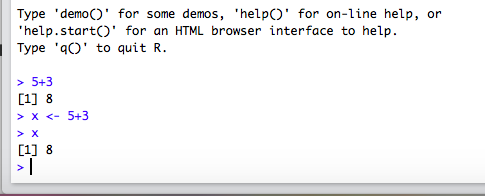
\includegraphics[width=7.29167in,height=\textheight,keepaspectratio]{more/rascalc.png}

\section{Saving your work}\label{saving-your-work}

Anything that you could ever want to accomplish in R can be done
directly in the console. However, if you are writing commands that you
might want to save for later or share with others, it is better to write
these inside a file, rather than in the console. For example, if you are
working on an assignment, you probably want to be able to access your
code again later to check your work.

The most basic type of file is an R Script file. You can create one by
going to File, New File, R Scipt. It should show up in the upper left
panel of your screen. This file works just like the console, but instead
of running a command every time you click enter, you can write several
lines at once without running them. If your cursor is on a certain line,
clicking ``run'' in the top right corner will execute just that line.
Clicking ``source'' will execute all lines at once. Experiment by typing
code such as the following into your R Script file. Make sure you are
comfortable with the difference between running an individual line and
running the whole file.

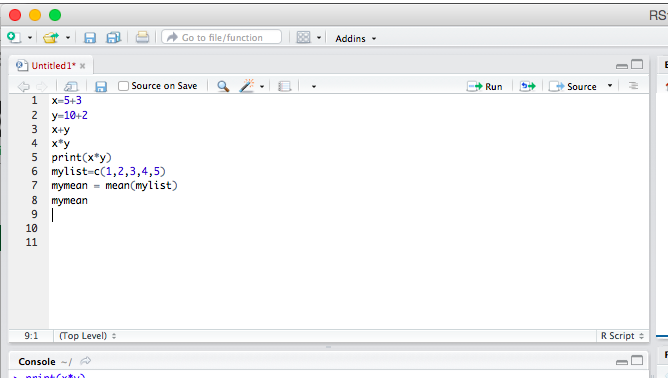
\includegraphics[width=7.29167in,height=\textheight,keepaspectratio]{more/RScriptpractice.png}

\begin{center}\rule{0.5\linewidth}{0.5pt}\end{center}

\subsection{RMarkdown files}\label{rmarkdown-files}

RScript files are great for code, but they are not great for
communicating your ideas to others. An RMarkdown file lets you
intersperse \emph{chunks} of R code with chunks of text and output the
result as a nicely formatted document. For all homework assignments in
this course, you will use RMarkdown to create documents that intersperse
code with answers to written discussion questions. We will typically
post the .Rmd file corresponding to the actual homework assignment, and
early in the semester you can use these files as \emph{templates}, where
all you need to do is fill in your answers. Later in the semester, for
your projects, you will need to be a bit more comfortable formatting
your own RMarkdown documents.

For today's tutorial, we will make an RMarkdown document from scratch.
In your RStudio application, select File, New File, R Markdown. If
prompted, select \texttt{PDF} as the default output format. Also, if
prompted to install any packages, please do so! You will know that you
were successful if you end up seeing an example file that looks like
this:

\includegraphics[width=9.375in,height=\textheight,keepaspectratio]{RMarkdown.png}

Anything written in this document on plain white background is
interpreted as text (write here as you would write in a Microsoft word
document), and any code written on gray background is interpreted as R
code (write here as you would write in the R console, with one command
per line). We call the gray areas \textbf{code chunks}.

Note that, when used on white background, the \texttt{\#} symbol creates
titles and headers that show up in large font in the output document. We
use text such as \texttt{\#\#\#\ Exercise\ 1} to label the exercises.
When used inside of a code chunk, the \texttt{\#} symbol in R creates a
code \textbf{comment}. This can be used to write regular text inside of
a code chunk. Any text written in a code chunk after the \texttt{\#}
symbol is ignored; it is not run as R code. We use comments to leave you
messages inside of lab and HW templates, such as ``write your answer
here''.

\emph{Knitting} an RMarkdown document means turning the input file
(\texttt{.Rmd}) into a nicely formatted output file (\texttt{.pdf} in
this case). To knit your current template document, select \texttt{knit}
from the buttons at the top of the RMarkdown file. A nicely formatted
document will open up in a new window.

Modify your example document so that it looks something like this one:

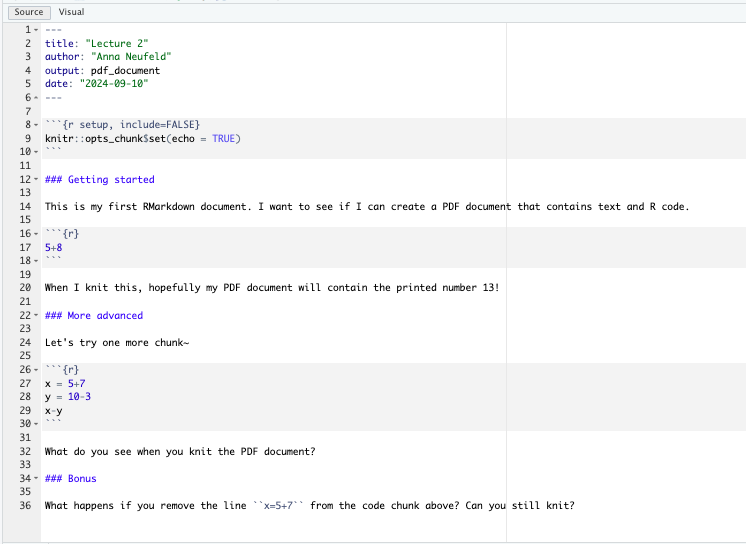
\includegraphics[width=9.375in,height=\textheight,keepaspectratio]{RMarkdown2.png}

\subsection{Running code in RMarkdown
files}\label{running-code-in-rmarkdown-files}

You will notice that just typing the code in the gray chunk did not
produce any sort of answer for us. To see the answer to this math
expression, we need to \textbf{run} this code.

\pandocbounded{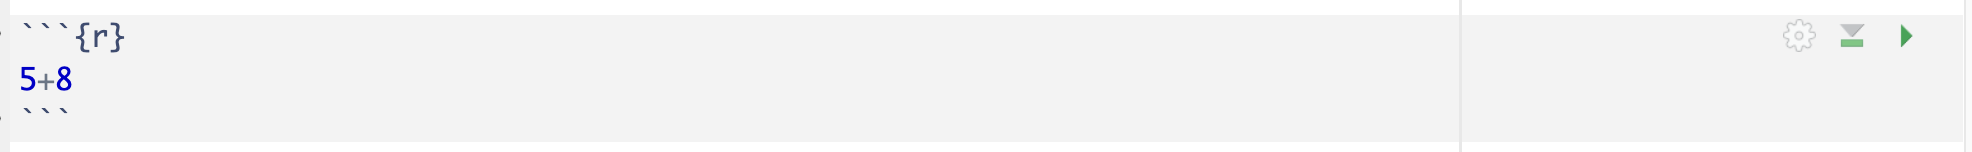
\includegraphics[keepaspectratio]{example.png}} First
note that all code in your chunks is automatically run each time you
knit your document. Knit your template document now to try this out! Did
it print your answer?

You can knit your R Markdown file every time you write code, but
sometimes the knitting process takes a few minutes and you just want to
run a few lines at a time to make sure they are working. To run chunks
without knitting, you can use either the Run button on the chunk (green
sideways triangle) or you can highlight the code and click Run on the
top right corner of the R Markdown editor. While it is good to run
individual chunks to test out ideas and explore, we also strongly
recommend that you \textbf{knit your document} each time you finish an
exercise. The knitting process can sometimes lead to errors. Students
often run in to trouble if they wait to try knitting their document
until right before the assignment deadline. Knitting after each exercise
ensures that you catch errors as you go.

When an R Markdown document is knitting, it only has access to the
variables that are created inside of the R Markdown document itself. The
R Markdown document does not get to use the environment in the upper
right hand corner of your screen while it is knitting. The R Markdown
document only gets to see the variables that are defined inside of the
document.

To illustrate this concept, delete the line
\texttt{x\ \textless{}-\ 5+7} from your sample document. Can you still
run the chunk locally? What happens if you try to knit your document?

\begin{Shaded}
\begin{Highlighting}[]
\NormalTok{y }\OtherTok{\textless{}{-}} \DecValTok{10{-}3}
\NormalTok{x}\SpecialCharTok{{-}}\NormalTok{y}
\end{Highlighting}
\end{Shaded}

It is also important in an R Markdown document that all variables are
defined in order. You will notice that exercise 5 contains two code
chunks in your template. What happens if you add
\texttt{x\ \textless{}-\ 5+7} back into your sample document, but you
add it to its own code chunk. Can you knit the document now?

\begin{center}\rule{0.5\linewidth}{0.5pt}\end{center}

\section{Loading and cleaning our first
dataset}\label{loading-and-cleaning-our-first-dataset}

While using R as a calculator was a fun warmup, in this class we are
typically going to use R to analyze datasets. With this in mind, we need
to learn how to load our dataset into R. There are several ways that we
will do this in this class.

\begin{itemize}
\tightlist
\item
  Many datasets are built into packages. These are extremely easy to
  load. As long as you have the package installed, you just load the
  package and then access the relevant dataset with the \texttt{data()}
  function. This is what you will be doing on HW1! These are typically
  datasets that are meant for educational purposes.
\item
  We can also load data in from an Excel file or a .csv file. This is
  probably the way that many of you will load your data for your final
  projects. You can do this using the \texttt{import\ dataset} button,
  which you will find in the top right corner of your RStudio interface.
\item
  Today, we will load our dataset directly from a URL. I sometimes post
  the dataset on my github website for you to read directly, because
  this is easier and quicker than uploading/downloading files. But this
  is sort of contrived because I post it in a really special format: you
  won't typically be able to do this in the real world.
\item
  Sometimes (later in the semester) we will generate our own data!
\end{itemize}

At the start of the semester, we will always give you very clear
instructions on how to load the required dataset. Eventually, for your
projects, you will need to know how to troubleshoot and load the data
yourself!

\subsubsection{Loading the ``Getting to Know You''
dataset}\label{loading-the-getting-to-know-you-dataset}

Over the weekend, 41 Stat 202 students filled out the ``getting to know
you'' survey. Google forms lets me export the survey responses into a
google sheet / Excel spreadsheet. I removed the names, pronouns, and
email addresses from the spreadsheet, and I also removed the answers to
the ``free response'' questions (e.g.~``Why are you taking this
class''). I changed the column names for readability. Finally, I saved
the resulting spreadsheet as a \texttt{.csv}.

As a very quick interlude on data ethics: I also removed \texttt{year}
at Williams. Since we only have two high school students in the class,
the data is hardly anonymous if you include this information! It is
always good to think about these things when preparing data to share!

I saved the anonymized data as a \texttt{.csv} file. I posted it both on
GLOW and on my github website. There are two ways that you can load the
data. The easiest is to run this code:

\begin{Shaded}
\begin{Highlighting}[]
\NormalTok{form\_data }\OtherTok{\textless{}{-}} \FunctionTok{read.csv}\NormalTok{(}\StringTok{"https://anna{-}neufeld.github.io/stat202\_tutorials/Week1/form\_data\_anonymous.csv"}\NormalTok{)}
\end{Highlighting}
\end{Shaded}

The slightly more cumbersome (but useful!) way involves downloading the
.csv document from GLOW and importing it using the
\texttt{import\ dataset} button. We will go over this later in the
semester.

Copy the code above into your RMarkdown document. Run the code, such
that you have an object called \texttt{form\_data} in your environment?
What happens if you click on this dataset?

\subsubsection{Manipulating and cleaning this
dataset}\label{manipulating-and-cleaning-this-dataset}

\phantomsection\label{boxedtext}
\textbf{Goals:}

\begin{itemize}
\tightlist
\item
  Review the basic language of data analysis.
\item
  Review some challenges of data cleaning.
\item
  Get exposed to the following functions:

  \begin{itemize}
  \tightlist
  \item
    \texttt{select()}
  \item
    \texttt{filter()}
  \item
    \texttt{mutate()}
  \end{itemize}
\end{itemize}

Click on \texttt{form\_data} in your \emph{environment}. You should see
something like this:

\pandocbounded{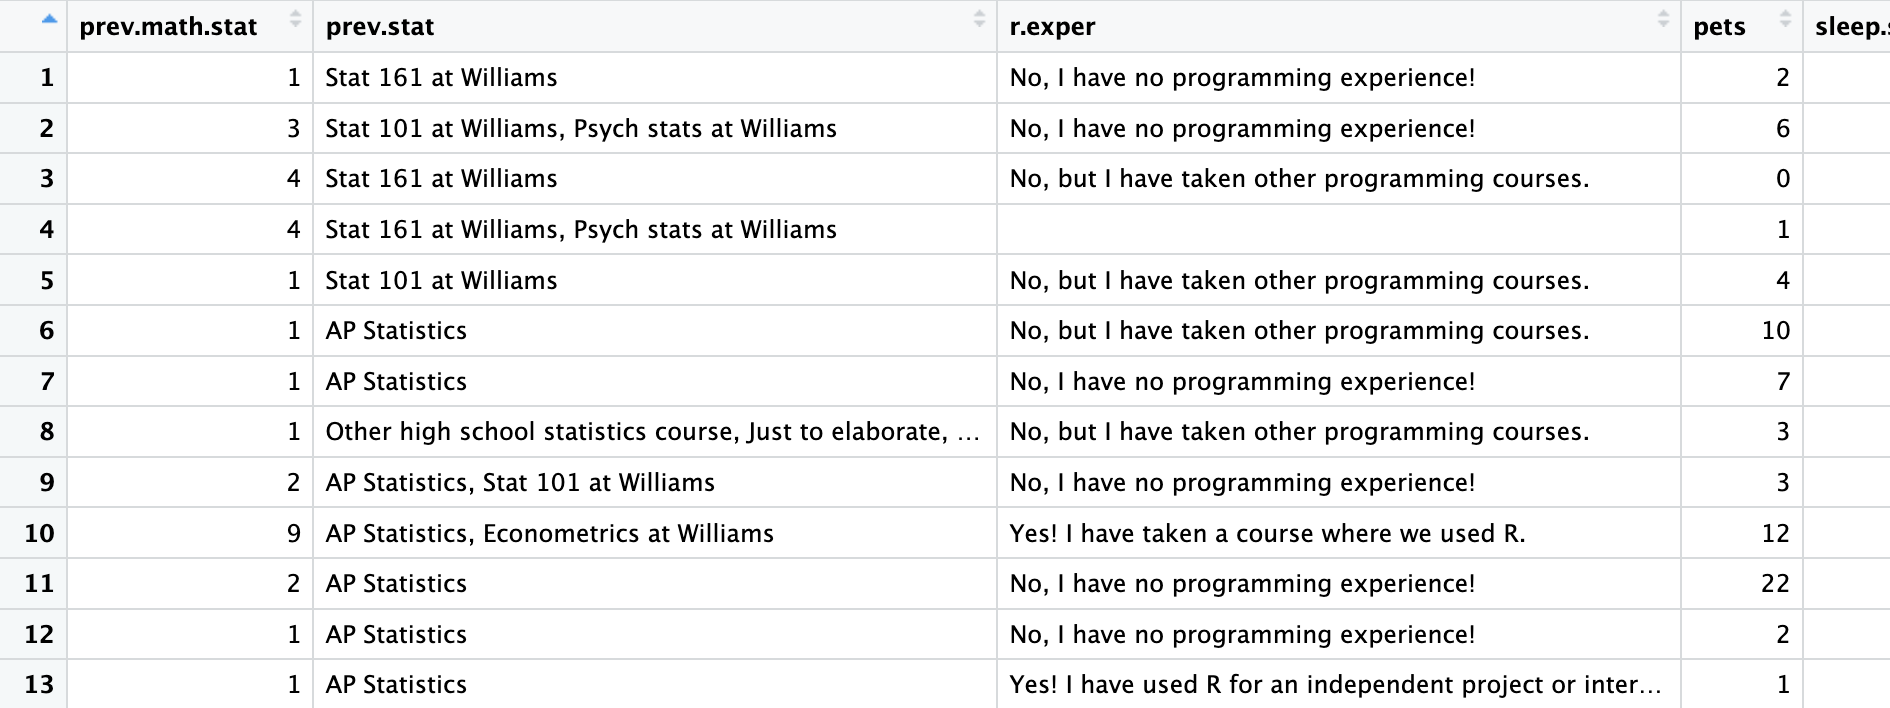
\includegraphics[keepaspectratio]{data.png}}

\phantomsection\label{boxedtext}
\textbf{With a neighbor, discuss the following questions:}

\begin{itemize}
\tightlist
\item
  What are the \textbf{observational units} in this dataset. How many
  are there?
\item
  What are some examples of \textbf{quantitative variables} in this
  dataset?
\item
  What are some examples of \textbf{categorical variables} in this
  dataset?

  \begin{itemize}
  \tightlist
  \item
    Bonus: are any of these \textbf{ordinal variables}?
  \end{itemize}
\item
  Do you see any issues with the data?
\end{itemize}

We are really lucky that we don't have too many issues with our data
this semester!

Last semester, many people added commentary to their numerical answers.
For example, these were all answers that I got last semester for ``How
many pets have you had or have you lived with in your life?'' on this
survey last semester.

\begin{itemize}
\tightlist
\item
  ``1! My dog Sammy is 8. He's a schnoodle.''
\item
  ``more than 25 fish, but no more than 7 at a time.''
\item
  ``3 dogs. 2 dogs currently''\\
\item
  ``2 cats!''
\end{itemize}

This led to some issues! I wanted this to be a numerical variable, but
\texttt{R} cannot figure out how to convert the sentence \emph{1! My dog
Sammy is 8. He's a schnoodle.} to a number automatically. This meant
that we had to spend a lot of time \emph{cleaning} our data. This
semester, I specifically asked you to enter the answer as a number, and
you all followed the instructions! This really reduced the number of
things that we will need to clean, which serves as a nice reminder for
me about the importance of survey design!

To see that we had issues with added commentary this year, we can
extract the \texttt{pets} variable from our dataset. There are a few
ways to do this. See if you can figure out any differences between
these.

\begin{Shaded}
\begin{Highlighting}[]
\NormalTok{form\_data}\SpecialCharTok{$}\NormalTok{pets}
\NormalTok{form\_data[,}\DecValTok{4}\NormalTok{]}
\NormalTok{form\_data }\SpecialCharTok{\%\textgreater{}\%} \FunctionTok{select}\NormalTok{(pets)}
\NormalTok{form\_data }\SpecialCharTok{\%\textgreater{}\%} \FunctionTok{pull}\NormalTok{(pets)}
\end{Highlighting}
\end{Shaded}

The function \texttt{select()} is a key function from the
\texttt{tidyverse()} package that we will be using to extract a subset
of \emph{variables} (columns) from a dataset.

When we want to select a subset of \emph{observations} (rows) from a
dataset, we use \texttt{filter()}. The following code displays only the
data for students who play a sport at Williams.

\begin{Shaded}
\begin{Highlighting}[]
\NormalTok{form\_data }\SpecialCharTok{\%\textgreater{}\%} \FunctionTok{filter}\NormalTok{(sports}\SpecialCharTok{==}\StringTok{"Yes"}\NormalTok{)}
\end{Highlighting}
\end{Shaded}

Suppose that we want to save the data subset above to a new dataset
called \texttt{athetes}. We can certainly do that!

\begin{Shaded}
\begin{Highlighting}[]
\NormalTok{athletes }\OtherTok{\textless{}{-}}\NormalTok{ form\_data }\SpecialCharTok{\%\textgreater{}\%} \FunctionTok{filter}\NormalTok{(sports}\SpecialCharTok{==}\StringTok{"Yes"}\NormalTok{)}
\end{Highlighting}
\end{Shaded}

One reason that the \texttt{tidyverse()} set of functions is so nice is
because it becomes quite easy to combine functions together. What does
the following code do?

\begin{Shaded}
\begin{Highlighting}[]
\NormalTok{form\_data }\SpecialCharTok{\%\textgreater{}\%} \FunctionTok{filter}\NormalTok{(sports}\SpecialCharTok{==}\StringTok{"Yes"}\NormalTok{) }\SpecialCharTok{\%\textgreater{}\%} \FunctionTok{select}\NormalTok{(pets)}
\end{Highlighting}
\end{Shaded}

And, as a harder question, why doesn't the following code work?

\begin{Shaded}
\begin{Highlighting}[]
\NormalTok{form\_data }\SpecialCharTok{\%\textgreater{}\%} \FunctionTok{select}\NormalTok{(pets) }\SpecialCharTok{\%\textgreater{}\%} \FunctionTok{filter}\NormalTok{(sports}\SpecialCharTok{==}\StringTok{"Yes"}\NormalTok{)}
\end{Highlighting}
\end{Shaded}

We do have one chance to do some data cleaning. Let's look at the
variable \texttt{favorite.coffee}.

\begin{Shaded}
\begin{Highlighting}[]
\NormalTok{form\_data}\SpecialCharTok{$}\NormalTok{favorite.coffee}
\end{Highlighting}
\end{Shaded}

While it is completely fine that some people do not drink coffee, we
probably do not want to treat ``n/a'', ``\,``, and''Don't Drink Coffee''
as separate answers. Furthermore, categorical variables with only one
category can be a bit hard to work with! Let's use the following code to
simplify this variable.

\begin{Shaded}
\begin{Highlighting}[]
\NormalTok{form\_data }\OtherTok{\textless{}{-}}\NormalTok{ form\_data }\SpecialCharTok{\%\textgreater{}\%} \FunctionTok{mutate}\NormalTok{(}\AttributeTok{favorite.coffee.clean =} \FunctionTok{ifelse}\NormalTok{(favorite.coffee }\SpecialCharTok{\%in\%} \FunctionTok{c}\NormalTok{(}\StringTok{"Tunnel"}\NormalTok{, }\StringTok{"Goodrich"}\NormalTok{), favorite.coffee, }\StringTok{"Other"}\NormalTok{))}
\end{Highlighting}
\end{Shaded}

We used \texttt{mutate} to make a new variable called
\texttt{favorite.coffee.clean}. This variable is equal to
\texttt{favorite.coffee} if \texttt{favorite.coffee} was equal to
\texttt{Tunnel} or \texttt{Goodrich}, but just stores \texttt{Other}
otherwise. Because we \emph{saved} our mutated dataset back into
\texttt{form\_data} (this step is very important!), we can now view our
new variable:

\begin{Shaded}
\begin{Highlighting}[]
\NormalTok{form\_data }\SpecialCharTok{\%\textgreater{}\%} \FunctionTok{select}\NormalTok{(favorite.coffee.clean)}
\end{Highlighting}
\end{Shaded}

I am sure that we will have many more chances to clean data later in the
semester!

\section{Exploratory Data Anlysis}\label{exploratory-data-anlysis}

\phantomsection\label{boxedtext}
\textbf{Goals:}

\begin{itemize}
\item
  Review the methods for numerically or visually summarizing different
  types of variables.
\item
  Get exposed to the following functions:

  \begin{itemize}
  \tightlist
  \item
    \texttt{group\_by()}
  \item
    \texttt{summarize()}
  \item
    \texttt{mean()}, \texttt{median()}, \texttt{sd()}, etc.
  \item
    \texttt{ggplot()}
  \item
    \texttt{geom\_histogram()}
  \item
    \texttt{geom\_boxplot()}
  \item
    \texttt{geom\_point()}
  \end{itemize}
\end{itemize}

When we do exploratory data analysis, we want to explore
\textbf{univariate} summaries of our individual variables. We also want
to explore \textbf{multivariate} relationships between our variables. We
want to do this visually, but we may also want to compute some summary
statistics! The type of visual and numerical summary depends on the type
of variable! We will dive into some examples below.

\subsubsection{One quantitative
variable}\label{one-quantitative-variable}

Let's use \texttt{pets,} which stores the recorded answers to the
question ``How many pets have you had or have you lived with in your
life?''.

Your are all familiar with many ways to summarize a single quantitative
variable. Most of these ways have really intuitive function names in
\texttt{R}. The \emph{summarize()} function is a nice way to view
multiple numeric summaries such as the mean and the median of a variable
at once. What do you notice about the mean number of pets as compared to
the median?

\begin{Shaded}
\begin{Highlighting}[]
\NormalTok{form\_data }\SpecialCharTok{\%\textgreater{}\%} \FunctionTok{summarize}\NormalTok{(}\FunctionTok{mean}\NormalTok{(pets), }\FunctionTok{median}\NormalTok{(pets))}
\end{Highlighting}
\end{Shaded}

While the mean and median are measures of \emph{center}, we might also
want to see some measures of \emph{spread}.

\begin{Shaded}
\begin{Highlighting}[]
\NormalTok{form\_data }\SpecialCharTok{\%\textgreater{}\%} \FunctionTok{summarize}\NormalTok{(}\FunctionTok{mean}\NormalTok{(pets), }\FunctionTok{median}\NormalTok{(pets), }\FunctionTok{sd}\NormalTok{(pets), }\FunctionTok{IQR}\NormalTok{(pets), }\FunctionTok{max}\NormalTok{(pets))}
\end{Highlighting}
\end{Shaded}

Note that each of these functions can be used individually without using
\texttt{summarize()}. But the main advantage of summarize is again that
it lets us view many summaries at once, and also it will be easy to
combine with functions like \texttt{filter()} and \texttt{mutate()}.

\begin{Shaded}
\begin{Highlighting}[]
\FunctionTok{mean}\NormalTok{(form\_data}\SpecialCharTok{$}\NormalTok{pets)}
\NormalTok{form\_data }\SpecialCharTok{\%\textgreater{}\%} \FunctionTok{pull}\NormalTok{(pets) }\SpecialCharTok{\%\textgreater{}\%} \FunctionTok{mean}\NormalTok{()}
\end{Highlighting}
\end{Shaded}

The best way to visually explore a single quantitative variable is with
a \emph{histogram}. There are two ways to make a histogram in
\texttt{R}.

\begin{Shaded}
\begin{Highlighting}[]
\FunctionTok{hist}\NormalTok{(form\_data}\SpecialCharTok{$}\NormalTok{pets)}
\end{Highlighting}
\end{Shaded}

In this class, we are going to focus on learning how to visualize and
summarize our data using the \texttt{tidyverse} suite of packages. As
part of this, we will be making plots using \texttt{ggplot()}. While at
first these may seem unnecessarily complex, they will eventually allow
you to make much more interesting and customizable plots than base R. I
use \texttt{ggplot()} for all of my research papers!

\begin{Shaded}
\begin{Highlighting}[]
\FunctionTok{ggplot}\NormalTok{(}\AttributeTok{data=}\NormalTok{form\_data, }\FunctionTok{aes}\NormalTok{(}\AttributeTok{x=}\NormalTok{pets))}\SpecialCharTok{+}\FunctionTok{geom\_histogram}\NormalTok{()}
\end{Highlighting}
\end{Shaded}

We can already start exploring the numerous ways that \texttt{ggplot()}
lets us customize our plots and make them beautiful.

\begin{Shaded}
\begin{Highlighting}[]
\FunctionTok{ggplot}\NormalTok{(}\AttributeTok{data=}\NormalTok{form\_data, }\FunctionTok{aes}\NormalTok{(}\AttributeTok{x=}\NormalTok{pets))}\SpecialCharTok{+}\FunctionTok{geom\_histogram}\NormalTok{(}\AttributeTok{bins=}\DecValTok{10}\NormalTok{)}\SpecialCharTok{+}
  \FunctionTok{xlab}\NormalTok{(}\StringTok{"How many pets have you lived with in your life?"}\NormalTok{)}\SpecialCharTok{+}
  \FunctionTok{ggtitle}\NormalTok{(}\StringTok{"Stat 202 Survey Responses about Pets"}\NormalTok{)}
\end{Highlighting}
\end{Shaded}

Finally, suppose that you want to visualize the number of pets, but only
among athletes at Williams. We can easily use the \emph{filter} function
to accomplish this; we just need to modify our \texttt{data} argument.

\begin{Shaded}
\begin{Highlighting}[]
\FunctionTok{ggplot}\NormalTok{(}\AttributeTok{data=}\NormalTok{form\_data }\SpecialCharTok{\%\textgreater{}\%} \FunctionTok{filter}\NormalTok{(sports}\SpecialCharTok{==}\StringTok{"Yes"}\NormalTok{), }\FunctionTok{aes}\NormalTok{(}\AttributeTok{x=}\NormalTok{pets))}\SpecialCharTok{+}\FunctionTok{geom\_histogram}\NormalTok{(}\AttributeTok{bins=}\DecValTok{10}\NormalTok{)}\SpecialCharTok{+}
  \FunctionTok{xlab}\NormalTok{(}\StringTok{"How many pets have you lived with in your life?"}\NormalTok{)}\SpecialCharTok{+}
  \FunctionTok{ggtitle}\NormalTok{(}\StringTok{"Stat 202 Survey Responses about Pets"}\NormalTok{, }\StringTok{"Among Athletes"}\NormalTok{)}
\end{Highlighting}
\end{Shaded}

\subsubsection{One categorical variable}\label{one-categorical-variable}

Suppose that we want to explore the variable \texttt{favorite.dining}.
This is a categorical variable.

Summarizing a single categorical variable is sort of boring! We don't
have measures of center and spread. The main way that we numerically
explore a single categorical variable is by making a table. Try out the
following lines of code, which all give the same information. What did
you learn about this variable?

\begin{Shaded}
\begin{Highlighting}[]
\NormalTok{form\_data }\SpecialCharTok{\%\textgreater{}\%} \FunctionTok{group\_by}\NormalTok{(favorite.dining) }\SpecialCharTok{\%\textgreater{}\%} \FunctionTok{summarize}\NormalTok{(}\FunctionTok{n}\NormalTok{())}
\FunctionTok{table}\NormalTok{(form\_data}\SpecialCharTok{$}\NormalTok{favorite.dining)}
\NormalTok{form\_data }\SpecialCharTok{\%\textgreater{}\%} \FunctionTok{select}\NormalTok{(favorite.dining) }\SpecialCharTok{\%\textgreater{}\%} \FunctionTok{table}\NormalTok{()}
\end{Highlighting}
\end{Shaded}

If we wanted to visually explore a single categorical variable, we would
typically use a bar chart. This displays the same information as the
table.

\begin{Shaded}
\begin{Highlighting}[]
\FunctionTok{ggplot}\NormalTok{(}\AttributeTok{data=}\NormalTok{form\_data, }\FunctionTok{aes}\NormalTok{(}\AttributeTok{x=}\NormalTok{favorite.dining))}\SpecialCharTok{+}\FunctionTok{geom\_bar}\NormalTok{()}
\end{Highlighting}
\end{Shaded}

\subsubsection{One quantitative variable, one categorical
variable.}\label{one-quantitative-variable-one-categorical-variable.}

Data analysis gets more interesting when we start looking at the
relationship between two or more variables. We need methods for
numerically or visually summarizing the relationships between variables.
Our methods will depend on what type of variables we are working with.
To start, suppose that we are working with one quantitative variable and
one categorical variable.

For example, suppose that we want to study the relationship between the
number of cups of coffee that someone drinks per week and whether or not
they play a sport at Williams. The best way to do this numerically is by
using \texttt{group\_by} and then \texttt{summarize}.

\begin{Shaded}
\begin{Highlighting}[]
\NormalTok{form\_data }\SpecialCharTok{\%\textgreater{}\%} \FunctionTok{group\_by}\NormalTok{(sports) }\SpecialCharTok{\%\textgreater{}\%} \FunctionTok{summarize}\NormalTok{(}\FunctionTok{mean}\NormalTok{(cups.coffee), }\FunctionTok{median}\NormalTok{(cups.coffee), }\FunctionTok{sd}\NormalTok{(cups.coffee), }\FunctionTok{n}\NormalTok{())}
\end{Highlighting}
\end{Shaded}

Note that this one person who answered both \texttt{Yes} and \texttt{No}
to the question of whether or not they play a sport at Williams is a bit
of an oddity. At the risk of throwing out valuable data, I am going to
remove them from the dataset! I can do this using \texttt{filter()}.

\begin{Shaded}
\begin{Highlighting}[]
\NormalTok{form\_data\_clean }\OtherTok{\textless{}{-}}\NormalTok{ form\_data }\SpecialCharTok{\%\textgreater{}\%} \FunctionTok{filter}\NormalTok{(sports}\SpecialCharTok{==}\StringTok{"Yes"} \SpecialCharTok{|}\NormalTok{ sports}\SpecialCharTok{==}\StringTok{"No"}\NormalTok{)}
\end{Highlighting}
\end{Shaded}

This takes our dataset and keeps only those who answered a simple
``Yes'' or ``No'' to the sports question. It then saves the filtered
dataset back to a new dataset called \texttt{form\_data\_clean}. This is
nice, because at least we know that our original dataset is not gone
forever.

We can now redo our summary table.

\begin{Shaded}
\begin{Highlighting}[]
\NormalTok{form\_data\_clean }\SpecialCharTok{\%\textgreater{}\%} \FunctionTok{group\_by}\NormalTok{(sports) }\SpecialCharTok{\%\textgreater{}\%} \FunctionTok{summarize}\NormalTok{(}\FunctionTok{mean}\NormalTok{(cups.coffee), }\FunctionTok{median}\NormalTok{(cups.coffee), }\FunctionTok{sd}\NormalTok{(cups.coffee), }\FunctionTok{n}\NormalTok{())}
\end{Highlighting}
\end{Shaded}

Based on this table, it does not seem like there is much of a
relationship between the amount of coffee that someone drinks and
whether or not they play a sport. Eventually in this class, we will
review statistical tools that will let us say more formally whether or
not there seems to be a relationship between these variables. For now,
we are just exploring and looking for patterns.

My favorite way to visually explore the relationship between one
categorical variable and one quantitative variable is with side-by-side
boxplots. The following code produces side-by-side boxplots with
\texttt{ggplot}. This boxplot again shows that there is likely no
relationship between sports and cups of coffee.

\begin{Shaded}
\begin{Highlighting}[]
\FunctionTok{ggplot}\NormalTok{(}\AttributeTok{data=}\NormalTok{form\_data\_clean, }\FunctionTok{aes}\NormalTok{(}\AttributeTok{x=}\NormalTok{sports, }\AttributeTok{y=}\NormalTok{cups.coffee))}\SpecialCharTok{+}\FunctionTok{geom\_boxplot}\NormalTok{()}
\end{Highlighting}
\end{Shaded}

\phantomsection\label{boxedtext}
\textbf{On your own: } Can you find a categorical variable and a
quantitative variable in this dataset that \emph{do} seem to be related
to one another? If so, what are they?

\subsubsection{Two quantitative
variables}\label{two-quantitative-variables}

When we want to look at the relationship between two quantitative
variables, we can use a scatterplot. We will be using a lot of
scatterplots later this semester! What do you notice about the
relationship below?

\begin{Shaded}
\begin{Highlighting}[]
\FunctionTok{ggplot}\NormalTok{(}\AttributeTok{data=}\NormalTok{form\_data, }\FunctionTok{aes}\NormalTok{(}\AttributeTok{x=}\NormalTok{sleep.semester, }\AttributeTok{y=}\NormalTok{cups.coffee))}\SpecialCharTok{+}\FunctionTok{geom\_point}\NormalTok{()}\SpecialCharTok{+}\FunctionTok{ylab}\NormalTok{(}\StringTok{"Average cups of coffee per week"}\NormalTok{)}\SpecialCharTok{+}\FunctionTok{xlab}\NormalTok{(}\StringTok{"Average hours of sleep per night during semester"}\NormalTok{)}\SpecialCharTok{+}\FunctionTok{ggtitle}\NormalTok{(}\StringTok{"Coffee vs. Sleep"}\NormalTok{)}\SpecialCharTok{+}\FunctionTok{theme\_bw}\NormalTok{()}
\end{Highlighting}
\end{Shaded}

When we want to numerically summarize the relationship between two
quantitative variables, we use correlation. According to the
correlation, there is a weak negative relationship between these two
variables. We will cover correlation in more depth later in the
semester!

\begin{Shaded}
\begin{Highlighting}[]
\FunctionTok{cor}\NormalTok{(form\_data}\SpecialCharTok{$}\NormalTok{sleep.semester, form\_data}\SpecialCharTok{$}\NormalTok{cups.coffee)}
\end{Highlighting}
\end{Shaded}

\subsubsection{Two categorical
variables}\label{two-categorical-variables}

In this final section, we will look at the relationship between a
student's favorite dining hall and what side of route 2 they live on.
Both of these variables are categorical. What do you notice from the
following table?

\begin{Shaded}
\begin{Highlighting}[]
\NormalTok{form\_data }\SpecialCharTok{\%\textgreater{}\%} \FunctionTok{select}\NormalTok{(route2.side, favorite.dining) }\SpecialCharTok{\%\textgreater{}\%} \FunctionTok{table}\NormalTok{()}
\end{Highlighting}
\end{Shaded}

Two-way tables are a great way to summarize the relationship between two
categorical variables. But there are actually a lot of subtle things
that we need to remember from intro stats. For example, if we want to
turn the counts in the table above into percentages, we actually have a
lot of choices about how to do this.

Consider the three tables below. Can you figure out what each one is
telling you? How do they differ? Which are most useful for studying the
relationhip between these two variables?

\begin{Shaded}
\begin{Highlighting}[]
\NormalTok{form\_data }\SpecialCharTok{\%\textgreater{}\%} \FunctionTok{select}\NormalTok{(route2.side, favorite.dining) }\SpecialCharTok{\%\textgreater{}\%} \FunctionTok{table}\NormalTok{() }\SpecialCharTok{\%\textgreater{}\%} \FunctionTok{prop.table}\NormalTok{()}
\NormalTok{form\_data }\SpecialCharTok{\%\textgreater{}\%} \FunctionTok{select}\NormalTok{(route2.side, favorite.dining) }\SpecialCharTok{\%\textgreater{}\%} \FunctionTok{table}\NormalTok{() }\SpecialCharTok{\%\textgreater{}\%} \FunctionTok{prop.table}\NormalTok{(}\AttributeTok{margin=}\DecValTok{1}\NormalTok{)}
\NormalTok{form\_data }\SpecialCharTok{\%\textgreater{}\%} \FunctionTok{select}\NormalTok{(route2.side, favorite.dining) }\SpecialCharTok{\%\textgreater{}\%} \FunctionTok{table}\NormalTok{() }\SpecialCharTok{\%\textgreater{}\%} \FunctionTok{prop.table}\NormalTok{(}\AttributeTok{margin=}\DecValTok{2}\NormalTok{)}
\end{Highlighting}
\end{Shaded}

Each of the tables above also has a corresponding visual that we can
make. You will practice interpreting these tables and plots on HW2. For
now, consider the plot below to be a preview of what is to come. How
would you interpret this?

\begin{Shaded}
\begin{Highlighting}[]
\FunctionTok{ggplot}\NormalTok{(}\AttributeTok{data=}\NormalTok{form\_data, }\FunctionTok{aes}\NormalTok{(}\AttributeTok{x=}\NormalTok{route2.side, }\AttributeTok{fill=}\NormalTok{favorite.dining))}\SpecialCharTok{+}\FunctionTok{geom\_bar}\NormalTok{(}\AttributeTok{position=}\StringTok{"stack"}\NormalTok{)}
\end{Highlighting}
\end{Shaded}

Based on the summaries above, do you think that there is a meaningful
relationship between a students' favorite dining hall and what side of
route 2 they live on? Discuss with your group!

\section{Wrap up}\label{wrap-up}

Hopefully, when you work on HW1, you will find that I went over all of
the R functions that you need for the homework in class. It is my goal
that this will be the case for every homework throughout the semester!

If you are already experienced in programming, I would encourage you to
go above-and-beyond on the homework assignments in terms of making your
code and your plots beautiful. If you are new to programming, please let
me know if the pacing seems too fast for you! I am happy to provide
additional resources for learning R if needed!

\begin{center}\rule{0.5\linewidth}{0.5pt}\end{center}

\subsection{Acknowledgements}\label{acknowledgements}

The formatting and some of the introductory content in this tutorial was
adopted from an OpenIntro lab.

\phantomsection\label{license}
This is a product of OpenIntro that is released under a
\href{http://creativecommons.org/licenses/by-sa/3.0}{Creative Commons
Attribution-ShareAlike 3.0 Unported}. This lab was adapted for OpenIntro
by Andrew Bray and Mine Çetinkaya-Rundel from a lab written by Mark
Hansen of UCLA Statistics.

\end{document}
